\documentclass[tikz,border=10pt]{standalone}
% Shared style for all project diagrams
\usepackage{amsmath,amssymb}
\usetikzlibrary{positioning,arrows.meta,calc,fit,decorations.pathreplacing}
\renewcommand{\familydefault}{\sfdefault}
\definecolor{accent}{RGB}{42,120,214}
\definecolor{lblue}{RGB}{234,242,252}
\definecolor{card}{RGB}{247,247,245}
\definecolor{ink}{RGB}{17,17,17}
\definecolor{gray52}{RGB}{82,81,78}
\definecolor{dblue}{RGB}{13,54,107}
\tikzset{
  box/.style={draw=accent, thick, rounded corners=3pt, fill=lblue, align=center,
              minimum height=1.05cm, inner sep=6pt, text=ink},
  plain/.style={draw=gray52!60, thick, rounded corners=3pt, fill=card, align=center,
              minimum height=1.05cm, inner sep=6pt, text=ink},
  ghost/.style={align=center, text=gray52, font=\footnotesize},
  arr/.style={-{Stealth[length=2.6mm]}, very thick, draw=accent},
  garr/.style={-{Stealth[length=2.6mm]}, thick, draw=gray52},
  lbl/.style={font=\footnotesize, text=gray52, align=center},
}

\begin{document}
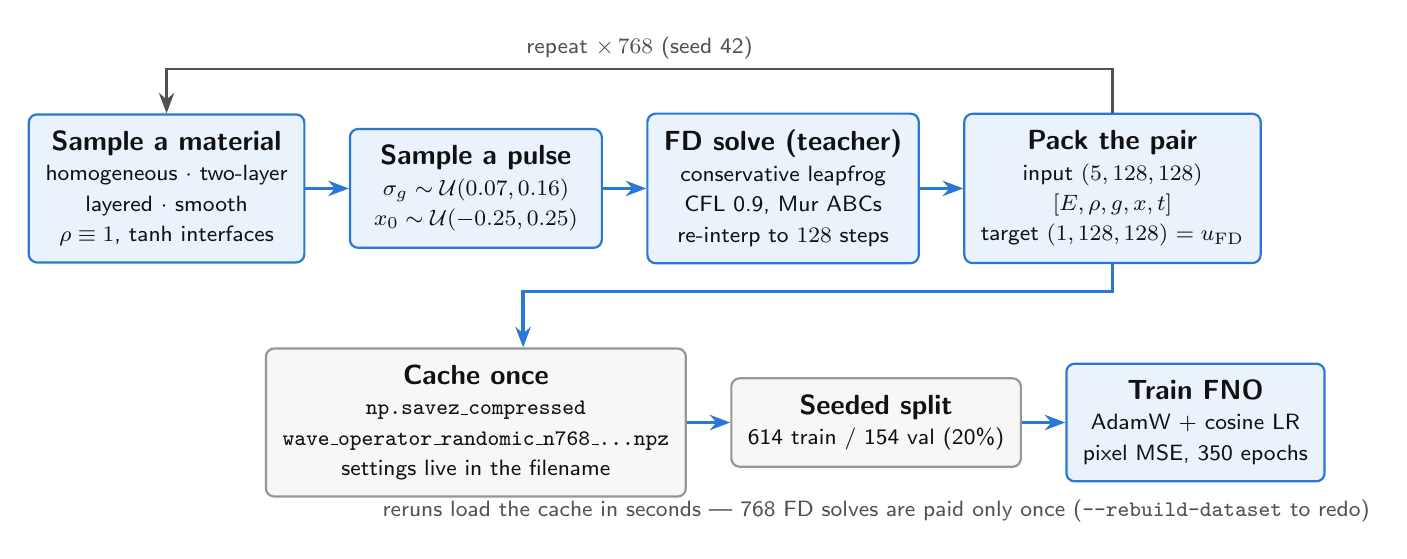
\begin{tikzpicture}[node distance=0.55cm and 0.55cm]
  \node[box, minimum width=3.5cm] (mat)
    {\textbf{Sample a material}\\[-1pt]
     {\footnotesize homogeneous $\cdot$ two-layer}\\[-1pt]
     {\footnotesize layered $\cdot$ smooth}\\[-1pt]
     {\footnotesize $\rho\equiv1$, tanh interfaces}};
  \node[box, right=of mat, minimum width=3.2cm] (ic)
    {\textbf{Sample a pulse}\\[-1pt]
     {\footnotesize $\sigma_g\sim\mathcal{U}(0.07,0.16)$}\\[-1pt]
     {\footnotesize $x_0\sim\mathcal{U}(-0.25,0.25)$}};
  \node[box, right=of ic, minimum width=3.4cm] (fd)
    {\textbf{FD solve (teacher)}\\[-1pt]
     {\footnotesize conservative leapfrog}\\[-1pt]
     {\footnotesize CFL 0.9, Mur ABCs}\\[-1pt]
     {\footnotesize re-interp to $128$ steps}};
  \node[box, right=of fd, minimum width=3.6cm] (pack)
    {\textbf{Pack the pair}\\[-1pt]
     {\footnotesize input $(5,128,128)$}\\[-1pt]
     {\footnotesize $[E,\rho,g,x,t]$}\\[-1pt]
     {\footnotesize target $(1,128,128)$ $=u_{\mathrm{FD}}$}};

  \draw[arr] (mat) -- (ic);
  \draw[arr] (ic) -- (fd);
  \draw[arr] (fd) -- (pack);

  % repeat loop
  \draw[garr] (pack.north) -- ++(0,0.55) -| (mat.north)
      node[pos=0.25, lbl, above] {repeat $\times\,768$ (seed 42)};

  % second row
  \node[plain, below=1.25cm of ic, minimum width=4.2cm] (cache)
    {\textbf{Cache once}\\[-1pt]
     {\footnotesize \texttt{np.savez\_compressed}}\\[-1pt]
     {\footnotesize \texttt{wave\_operator\_randomic\_n768\_...npz}}\\[-1pt]
     {\footnotesize settings live in the filename}};
  \node[plain, right=of cache, minimum width=3.0cm] (split)
    {\textbf{Seeded split}\\[-1pt]
     {\footnotesize 614 train / 154 val (20\%)}};
  \node[box, right=of split, minimum width=3.2cm] (train)
    {\textbf{Train FNO}\\[-1pt]
     {\footnotesize AdamW + cosine LR}\\[-1pt]
     {\footnotesize pixel MSE, 350 epochs}};

  \draw[arr] (pack.south) -- ++(0,-0.35) -| ($(cache.north)+(0.6,0)$);
  \draw[arr] (cache) -- (split);
  \draw[arr] (split) -- (train);

  \node[lbl, below=0.28cm of split, xshift=0.0cm]
    {reruns load the cache in seconds --- 768 FD solves are paid only once (\texttt{--rebuild-dataset} to redo)};
\end{tikzpicture}
\end{document}
